% Chapter Template

\chapter{Localization System Implementation} % Main chapter title

\label{Chapter5} % Change X to a consecutive number; for referencing this chapter elsewhere, use \ref{ChapterX}
In this section we explain the hardware and software components of our system architecture in detail. Then we introduce the implementation of the different localization algorithm components and we describe the underlying UWB communication.

%----------------------------------------------------------------------------------------
%	SECTION 1
%----------------------------------------------------------------------------------------

\section{Localization Components Hardware}
The four different hardware components - server, client, ANs and APs - that were important in our implementation are already shown in Figure \ref{fig:system_components} of the last chapter. In the following we explain which explicit hardware we used for our experiments.\\
\noindent\hspace*{5mm}%
Our proposed algorithm was running on a commodity laptop, which was used as our server, connected via Ethernet to a sink anchor node. The laptop was a low to mid-end commercial notebook with fairly limited computational power.\\
\noindent\hspace*{5mm}%
The target device was a Raspberry Pi Model B \cite{Raspberry} with a 1.2 GHz 64-bit CPU running the operating system Raspian. On the 40 pin GPIO, it was equipped with a Sequitur InGPS Lite Tag Chip from UNISET to enable UWB communication as well as acceleration and magnetic field measurements.\\
\noindent\hspace*{5mm}%
The sink node and the other anchor nodes were also Raspberry Pi Model B with the same specifications. However, the ANs were not equipped with a TAG Chip, but with a Sequitur InGPS Lite Anchor Chip, exclusively enabling UWB communication.\\
\noindent\hspace*{5mm}%
For the WiFi access points, we used several commercial commodity access points from D-Link (D-635 and DAP-2553).\\
\noindent\hspace*{5mm}%
The detailed specification of each component is summarized in Table \ref{tab:hardware_specification}.
\begin{table}
\caption{Hardware Components}
\label{tab:hardware_specification}
\centering
\begin{tabular}{| c | c |}
\toprule
\textbf{Device} & \textbf{Model}\\
\midrule
& \textbf{Model:} HP EliteBook\\
Server & \textbf{CPU:} 2.30 GHz Intel Core i5-5300U\\
& \textbf{Architecture:} 64-bit\\
& \textbf{OS:} Windows 10 Enterprise\\
& \textbf{RAM:} 8 GB\\
\midrule
& \textbf{Model:} Raspberry Pi Model B\\
Target & \textbf{CPU:} Quad Core 1.2GHz\\
& \textbf{Architecture:} 64-bit\\
& \textbf{OS:} Raspbian 4.14\\
& \textbf{RAM:} 1 GB\\
& \textbf{WLAN:} WiFi b/g/n\\
& \textbf{Extension:} Sequitur Pi (InGPS Lite Tag)\\
\midrule
& \textbf{Model:} Raspberry Pi Model B\\
Anchors & \textbf{CPU:} Quad Core 1.2GHz\\
& \textbf{Architecture:} 64-bit\\
& \textbf{OS:} Raspbian 4.14\\
& \textbf{RAM:} 1 GB\\
& \textbf{WLAN:} WiFi b/g/n (not used)\\
& \textbf{Extension:} Sequitur Pi (InGPS Lite Anchor)\\
\midrule
& \textbf{Model:} Sequitur Pi (InGPS Lite)\\
Ultra WideBand Extention & \textbf{Ultra WideBand:} IEEE 802.15.4a\\
& \textbf{IMU (tag only):} 3D-Accelerometer, 3D-Magnetometer\\
& \textbf{Firmware:} Sequitur InGPS Lite Anchor/Tag (from UNISET)\\
\bottomrule
\end{tabular}
\end{table}

%----------------------------------------------------------------------------------------
%	SECTION 2
%----------------------------------------------------------------------------------------

\section{Localization Components Software}
The localization algorithm was configured with a minimal update period of 0.7 seconds. This means, that the system triggered all input sources and performed all three particle filter phases, such that every 0.7 seconds a position estimation was provided. However, in some cases, the update time was longer, when it took more time to fetch data from the data sources. The position estimation was done based on 100 particles.\\
\noindent\hspace*{5mm}%
The motion vector was calculated by using the velocity of the device in the last system update. This velocity was turned to the measured heading direction and adapted by the obtained acceleration.  As the sample rate of the accelerometer sensor was 10 Hz, for each system state update we had seven or more discrete acceleration measurements, we stored these measurements in the client device until the server requested the movement vector. As the acceleration sensor - depending on pitch and roll of the device - had a huge non-zero mean noise, we decided to not use the accelerometer data directly, but to use the change in acceleration. The advantage of this implementation was, that errors of acceleration measurements due to pitch, roll and tilt of the device were only registered in a small period of time and not constantly. In the other hand it had the downside that constant acceleration was not detected correctly, however a constant acceleration is occuring less often than a tilted device when tracking a pedestrian. To gather the change in acceleration we fed the sensor data into two low pass filters with different parameters, one with a high adaption of 0.98 and one with a low adaption of 0.03, and only took their difference into account. This means we calculated the difference between $a_{t}^1$ and $a_{t}^2$, which were calculated as in \ref{eqn:a1} and \ref{eqn:a2}:
\begin{equation}
a_{t}^{1} = \hat{a}_{t}*0.03 + a_{t-1}^{1} * 0.97
\label{eqn:a1}
\end{equation}
and
\begin{equation}
a_{t}^{2} = \hat{a}_{t}*0.98 + a_{t-1}^{2} * 0.02
\label{eqn:a2}
\end{equation}
with $\hat{a}_{t}$ as the measured acceleration in timeslot $t$, $a_{t-1}^{1}$ and $a_{t-1}^{2}$ the low pass filtered acceleration results in timeslot $t-1$ of the first and the second low pass filter respectively.\\
\noindent\hspace*{5mm}%
We read the floorplan information from an image of the floorplan. The image data was then stored in a matrix with values 0, if the position was not allowed, and any other value bigger than 0, when the position was an allowed position. For checking if a position was reachable, we started at the old position and checked if all values on the direct path between the old and the new position were bigger than 0. To get from the direct path to the discrete matrix positions, we used the commonly known algorithm called Bresenham's line algorithm \cite{bresenham}.\\
\noindent\hspace*{5mm}%
For gathering ranging information, the Sequitur InGPS Lite firmware provided a two-way ranging method. The range estimation of two nodes was triggered by the application programming interface (API) command $CLIENT\_GET\_RANGE\ (50)$. In our application, we sent the command to the anchor in order to minimize the communication of the TAG. The flow of actions related to this API is an even more simplified version of the message exchange indicated in Figure \ref{fig:two_way_ranging}. In our case, the request message performed by the server started the TWR conversation via UWB between AN and TAG. The AN sent only one ranging request to the TAG, which immediately responded. This simplified version of TWR is illustrated in Figure \ref{fig:simple_TWR}. By observing the difference between the time instants related to the transmission of the request packet and the reception of the response packet, the AN directly determined the RTT and thus the range.  Finally, an answer message with the range was reported from the AN to the server and no messages were reported from the TAG to the server.\\
\noindent\hspace*{5mm}%
The zone indication fused Wi-Fi and UWB RSS in an enhanced ensemble learning model, which means that not only one machine learning algorithm was used, but a combination of several different machine learning algorithms. In our zone indication, a set of independent individual machine learning algorithms were fed with the same fingerprint data. Every machine learning algorithms performed a zone prediction and assigned a likelihood to every zone. The likelihood represented the probability of observing the given RSS fingerprint while being in this zone. We assumed that for every machine learning algorithm these probabilities were statistically independent, thus the probabilities returned by our ensemble learning algorithm were just the multiplied results of the single machine learning algorithms.\\
We used these three completely different ML algorithms: Decision Tree Learning with gini impurity \cite{WikiGini}, K nearest neighbor (KNN) classification \cite{KNN} and a soft voting classifier using gini, KNN and gaussian naive bayes \cite{SKLearn, GaussianNB} algorithms. We selected these three algorithms out of half a dozen machine learning algorithms, because those three had the best classification results in the test data. For the testing data, the three machine learning algorithms had a correct prediction rate of 80 to 99 percent. 

\begin{figure}[th]
\centering
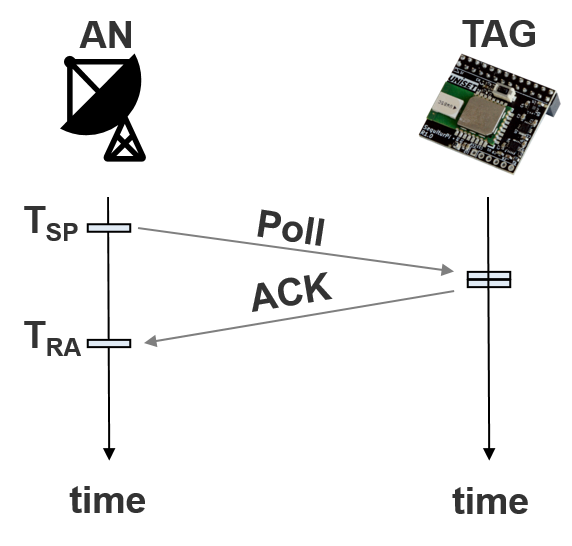
\includegraphics[width=0.6\textwidth]{Figures/simple_TWR}
\decoRule
\caption[Minimal Two Way Ranging]{Minimal implementation of two way ranging.}
\label{fig:simple_TWR}
\end{figure}

%----------------------------------------------------------------------------------------
%	SECTION 3
%----------------------------------------------------------------------------------------

\section{Ultra Wideband Communication}
The radio module of the Sequitur Pi board was not only used  to evaluate the ToF but also to transmit data to the server via the sink anchor node, in order to avoid the need for additional communication hardware. As UNISET is a commercial company, they do not provide full information of the implemented transmission techniques. Nonetheless, in the following, we mention the known parts and the configuration parameters.\\
\noindent\hspace*{5mm}%
Sequitur InGPS Lite enables single-hop wireless communication with the UWB interface between neighboring nodes of the same network. The radio module supports different user-selectable frequency bands between 3.5 GHz and 6.5 GHz. There are six different operation modes to change the spectral occupation, listed in table \ref{tab:spectral_occupation}.\\
\begin{table}
\caption{Spectral Occupation of Predefined Channels.}
\label{tab:spectral_occupation}
\centering
\begin{tabular}{c c c}
\toprule
\textbf{Channel Number} & \textbf{Central Frequency}[MHz] & \textbf{Bandwidth}[MHz]\\
\midrule
1 & 3494.4 & 500\\
2 & 3993.6 & 500\\
3 & 4492.8 & 500\\
4 & 3993.6 & 1300\\
5 & 6489.6 & 500\\
7 & 6489.6 & 1100\\
\bottomrule\\
\end{tabular}
\end{table}
The data rate can be changed to three preset values of 110 kbps, 850 kbps and 6.8 Mbps. All nodes have to operate in the same radio mode and frequency band to communicate correctly. In general, a lower data rate allows larger operating distances between the nodes. The transmission power of the radio module could be selected between 1 and 63, whereas 63 is the highest value. Every number increases the transmitting power by 0.5 dB. The default pulse repetition frequency (PRF) is assumed to be 64 MHz for all the channels. The underlying modulation techniques are not indicated in the specifications \cite{Usermanual, Beginnersguide}.\\
\noindent\hspace*{5mm}%
In our implementation the UWB transmitters of all UWB devices operated in radio mode 2 with a data rate of 850 kbps, were configured to use channel 4 with a central frequency of 3993.6 MHz and an occupied spectrum of 1300 MHz. The transmission power was set to a maximum of 63 and the PRF to the default value of 64 MHz. Before starting the experiments, a 15-meter calibration with 1000 measurements per device was made as described in the beginner's guide \cite{Beginnersguide}.